\section{Sprint Backlog}

\subsection{User Stories del Primer Sprint}

\fbox{\parbox{\textwidth}{%
	{\LARGE\bf User Story 1} \hfill Story Points: \textbf{5.0} \\
	Como administrador quiero poder simular una acción ofensiva y defensiva.
	\begin{description}
		\item [Descripción] Cada turno está separado en varias partes, y en cada parte los equipos dos equipos tiene asignados una acción ofensiva, y una defensiva. Hay que poder simular por lo menos uno de estos casos para poder probar el sistema de juego.
		\item [Criterios de Aceptación] Las dos jugadas son razonablemente complejas, y que funcionan lo suficientemente bien para construir la primer parte del sistema al rededor de ellas.

		\item \fbox{\parbox{.96\textwidth}{
			{\Large\bf Tarea 1} \hfill Horas hombre: \textbf{14.0} \vspace{1ex} \\
			\textbf{Descripción} Crear una acción ofensiva
		}}

		\item \fbox{\parbox{.96\textwidth}{
			{\Large\bf Tarea 2} \hfill Horas hombre: \textbf{14.0} \vspace{1ex} \\
			\textbf{Descripción} Crear una acción defensiva
		}}
	\end{description}
}}

\fbox{\parbox{\textwidth}{%
	{\LARGE\bf User Story 2} \hfill Story Points: \textbf{5.0} \\
	Como administrador quiero editar fórmulas y números  de resolución de acciones para poder cambiar el juego en caso de que se necesite.
	\begin{description}
		\item [Descripción] La probabilidad de que cada acción sea exitosa depende de unas fórmulas complejas que son dificiles de tener ``bien'' en la primera vez. Por eso es importante que sea fácil modificarlas aunque el producto esté más avanzado.
		\item [Criterios de Aceptación] Las fórmulas de una cantidad minimal de acciones deben estar implementadas, y deben ser facilmente editables.

		\item \fbox{\parbox{.96\textwidth}{
			{\Large\bf Tarea 1} \hfill Horas hombre: \textbf{8.0} \vspace{1ex} \\
			\textbf{Descripción} Crear fórmulas editables para primeras acciones.
		}}
	\end{description}
}}

\fbox{\parbox{\textwidth}{%
	{\LARGE\bf User Story 3} \hfill Story Points: \textbf{16.0} \\
	Como participante quiero ver log del partido e información pertinente para poder visualizar las simulaciones anteriores.
	\begin{description}
		\item [Descripción] Gran parte de la información sobre cuan bien funciona el sistema va a set descubierta con jugadas hechas por jugadores reales. Tener logs de jugadas anteriores es importante para conocer este proceso.
		\item [Criterios de Aceptación] El log minuto-a-minuto debe estar listo y presentar todas las acciones que pasan en varios partidos.

		\item \fbox{\parbox{.96\textwidth}{
			{\Large\bf Tarea 1} \hfill Horas hombre: \textbf{4.0} \vspace{1ex} \\
			\textbf{Descripción} Crear interfaz de mensajes con todos los objetos del partido.
		}}

		\item \fbox{\parbox{.96\textwidth}{
			{\Large\bf Tarea 2} \hfill Horas hombre: \textbf{10.0} \vspace{1ex} \\
			\textbf{Descripción} Lograr que el log pueda recibir bien esas llamadas y que no haya problemas con cosas como concurrencia.
		}}

		\item \fbox{\parbox{.96\textwidth}{
			{\Large\bf Tarea 3} \hfill Horas hombre: \textbf{6.0} \vspace{1ex} \\
			\textbf{Descripción} Interfacear con una base de datos para poder volcar el log a un medio consistente cuando termine un partido.
		}}
	\end{description}
}}

\fbox{\parbox{\textwidth}{%
	{\LARGE\bf User Story 4} \hfill Story Points: \textbf{2.0} \\
	Como participante quiero nombrar mi equipo, elegir mi jugador estrella y mi tecnico.
	\begin{description}
		\item [Descripción] Los participantes necesitan tener un mínimo nivel de customización con el juego, y poder elegir el nombre del equipo, el \textit{MVP}, y a quién usar como técnico es ideal.
		\item [Criterios de Aceptación] Cuando se crea un equipo nuevo se deben poder agregar esos tres datos.

		\item \fbox{\parbox{.95\textwidth}{
			{\Large\bf Tarea 1} \hfill Horas hombre: \textbf{2} \vspace{1ex} \\
			\textbf{Descripción} Crear una manera de cambiarle el nombre al equipo.
		}}

		\item \fbox{\parbox{.95\textwidth}{
			{\Large\bf Tarea 2} \hfill Horas hombre: \textbf{2} \vspace{1ex} \\
			\textbf{Descripción} Poder elegir, entre todos los jugadores del equipo, cuál es da real MVP.
		}}

		\item \fbox{\parbox{.95\textwidth}{
			{\Large\bf Tarea 3} \hfill Horas hombre: \textbf{2.0} \vspace{1ex} \\
			\textbf{Descripción} Lograr que el usuario pueda ver una lista de técnicos y que pueda elegir uno para su equipo.
		}}
	\end{description}
}}

\newpage

\subsection{Burndown Chart}
A continuación mostramos el gráfico del burndownchart que muestra las horas trabjadas a lo largo de 24 días que era lo estimado para terminar el primer sprint.

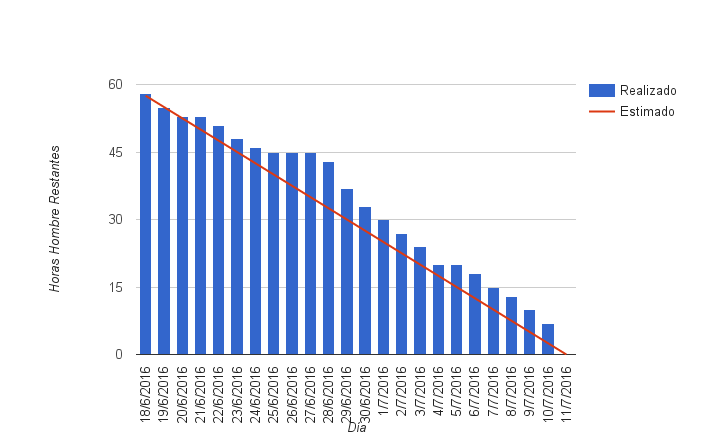
\includegraphics[width=\textwidth]{imgs/burndown.png}


% \textbf{Como participante quiero nombrar mi equipo, elegir mi jugador estrella y mi tecnico.} & \Large2&\Large5 \\ \hline
% 
% \subsection{Otras User Stories}
% Como participante quiero poder registrar una cuenta para acceder al juego. & \Large2 & \Large8  \\ \hline
% Como participante quiero buscar desafíos para poder aceptarlos. & \Large5 & \Large5 \\ \hline
% Como participante quiero armar equipos para poder aceptar o postular desafíos con ese equipo. & \Large3 & \Large5 \\ \hline
% Como administrador quiero administrar jugadores disponibles para poder organizar el juego. & \Large3 & \Large2 \\ \hline
% Como administrador quiero consultar las cuentas que están en el sistema para poder analizar el uso del juego por los participantes. & \Large5 & \Large2\\ \hline
% Como participante quiero autenticar mi cuenta (log in) para poder entrar en el sistema de juego. & \Large2 &\Large8 \\ \hline
% Como participante quiero poder ver mi cap y mis fichas para decidir mis apuestas. &\Large2 &\Large3 \\ \hline
% Como participante quiero ver tabla de posiciones de todos los participantes en base a sus desafíos ganados/perdidos para poder conocer el ranking. & \Large3 & \Large2\\ \hline
% Como participante quiero postular desafío para desafiar a otros participantes a que jueguen contra mi equipo. & \Large2 & \Large5 \\ \hline
% Como participante quiero aceptar el desafío postulado por otro participante para poder jugar contra otros equipos. & \Large2 & \Large5 \\ \hline
% Como administrador quiero poder crear jugadas ofensivas y defensivas. &\Large5&\Large3 \\ \hline
